\chapter{Ergebnisse und Diskussion}
Nachdem nun auf demselben Datensatz ein Modell mit nnU-Net und eines mit SegResnet trainiert wurden sollen im Folgenden die Ergebnisse aufgezeigt werden. 

\begin{table}[H]
\begin{tabular}{|c|c|c|c|c|}
\hline 
Modell & \multicolumn{4}{c|}{Dice-Score je Label} \\ 
\hline 
• & Edema & Non-Enhancing Tumor & Enhancing Tumor & Duchschnitt \\ 
\hline 
nnU-Net & 0.7770 & 0.5954 & 0.8003 & 0.7243 \\ 
\hline 
SegResNet & 0.7851 & 0.5645 & 0.7901 & 0.7133 \\ 
\hline 
\end{tabular} 
\caption{\label{tab:dice}Dice-Scores der Modelle je Label}
\end{table}

Wie in Tabelle \ref{tab:dice} zu sehen ist, erzielt nnU-Net ein leicht besseres Ergebnis. Lediglich bei der Segmentierung des Edema liegt das SegResNet minimal vorne. Jedoch denke ich das mit weiteren Optimierungen ein besseres Ergebnis erzielt werden könnte. Dies war mir im Rahmen der Studienarbeit aus zeitlichen Gründen leider nicht mehr möglich. Bevor ich das SegResNet trainiert hatte, habe ich einige Versuche mit dem SwinUNetr-Modell unternommen. Durch den begrenzten GPU-Speicher der Hochschulrechner war es mir mit diesem Modell leider nicht möglich vernünftige Ergebnisse zu erzielen weshalb ich diesen Ansatz verwarf. Jedoch stieß ich auch mit dem SegResNet an meine Grenzen, bis ich Zugriff zum GPU-Server erhielt. Leider ging dabei viel Zeit verloren die ich gerne noch in Anpassungen des SegResNet gesteckt hätte. Hinzu kommt, dass das Training des SegResNet etwa 24h+ dauerte und ein durch einen Neustart einige Ergebnisse verloren gingen und ich daher das Training erneut gestartet habe.

In Abbildung \ref{fig:resultnnunet} werden in der oberen Reihe die ursprünglichen Label angezeigt, in der unteren Reihe die Ergebnisse des Modells. Dasselbe gilt für Abbildung \ref{fig:resultsegresnet}.

\begin{figure}
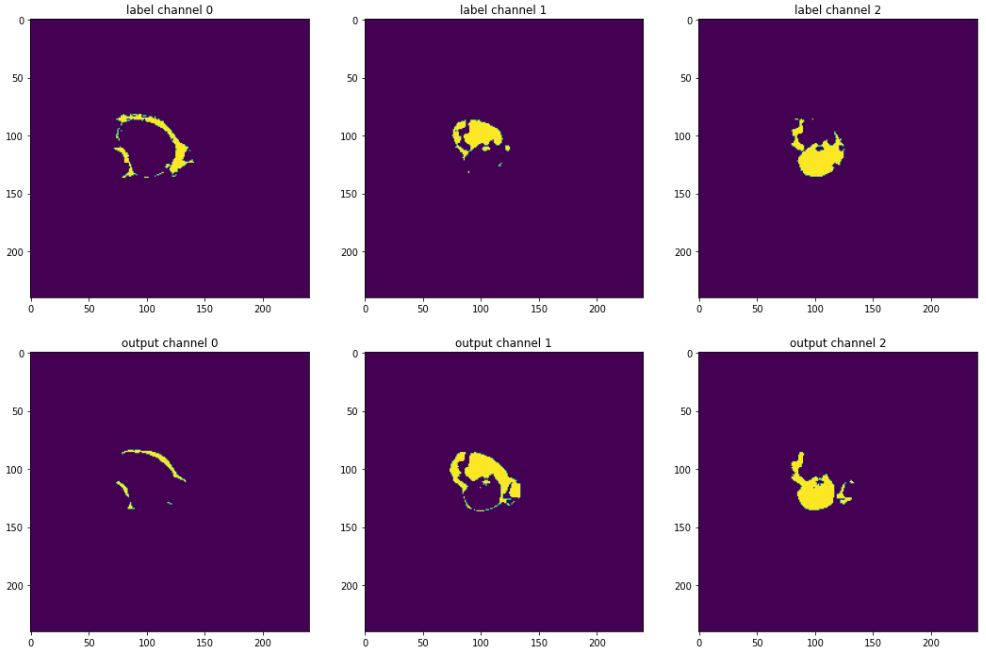
\includegraphics[width=\linewidth]{./images/nnunetresult.jpg}
\captionof{figure}{Ergebnis nnU-Net}
\label{fig:resultnnunet}
\end{figure}

\begin{figure}
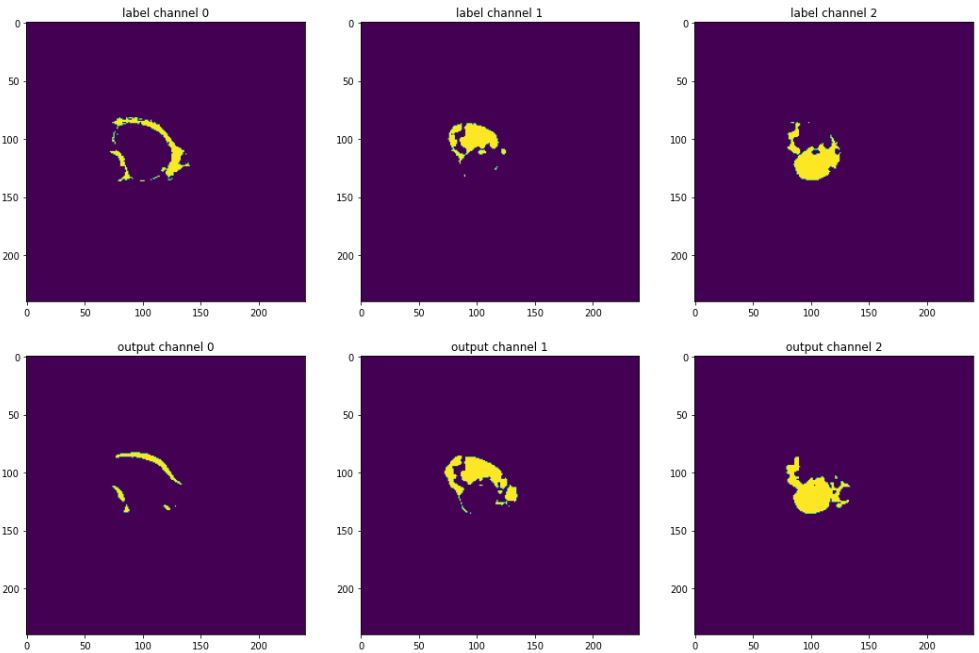
\includegraphics[width=\linewidth]{./images/resultsegresnet.jpg}
\captionof{figure}{Ergebnis SegResNet}
\label{fig:resultsegresnet}
\end{figure}

In Abbildung \ref{fig:segresnetmetrics} kann man den Trainingsverlauf des SegResNet sehen. Deutlich wird das die Ergebnisse erst ab Epoche 50 annehmbar sind. Ab Epoche 200 ist keine Verbesserung mehr zu erwarten. Das beste Ergebnis des SegResNet wurde in Epoche 197 erreicht. Zu nnU-Net liegen mir diese Daten leider nicht vor.
\begin{figure}[H]
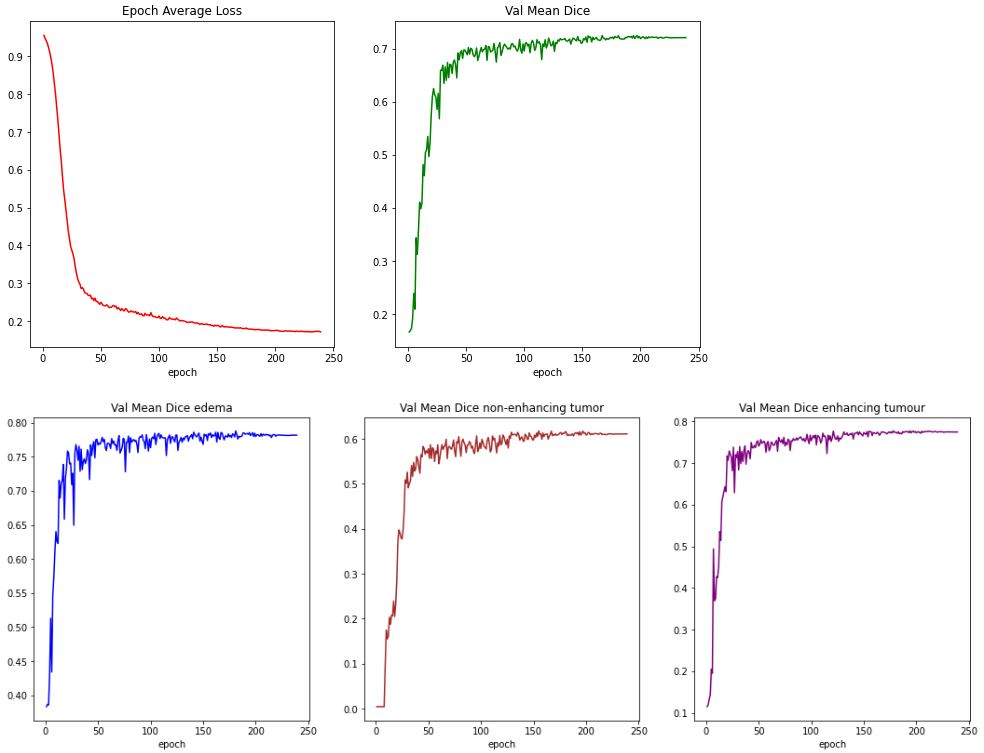
\includegraphics[width=\linewidth]{./images/segresnetmetrics.jpg}
\captionof{figure}{Trainingsverlauf SegResNet}
\label{fig:segresnetmetrics}
\end{figure}